\chapter{Tabelas Hash}
\chaplabel{hashtables}
\chaplabel{hashing}

As tabelas Hash são um método eficiente de armazenar um número pequeno, #n#, de números inteiros de uma grande faixa $U=\{0,\ldots,2^{#w#}-1\} $. O termo \emph{tabela hash}
\index{hash table} %
inclui uma ampla gama de estruturas de dados. A primeira parte deste capítulo concentra-se em duas das implementações mais comuns de tabelas de hash: hashing com encadeamento e sondagem linear.

Muitas vezes, as tabelas hash armazenam tipos de dados que não são inteiros. Nesse caso, um inteiro \emph{código hash}
\index{hash code}%
está associado a cada item de dados e é usado na tabela hash. A segunda parte deste capítulo discute como esses códigos de hash são gerados.

Alguns dos métodos utilizados neste capítulo exigem escolhas aleatórias de números inteiros em algum intervalo específico. Nos exemplos de código, alguns desses números inteiros ``aleatórios'' são constantes codificadas. Essas constantes foram obtidas usando bits aleatórios gerados pelo ruído atmosférico.


\section{#ChainedHashTable#: Uma Tabela de Dispersão por Encadeamento}
\seclabel{hashtable}

\index{ChainedHashTable@#ChainedHashTable#}%
\index{chaining}%
\index{hashing with chaining}%
Uma estrutura de dados #ChainedHashTable# usa \emph{dispersão por encadeamento} para armazenar dados como um array, #t#, de listas. Um número inteiro, #n#, acompanha o número total de itens em todas as listas (veja \figref{chainedhashtable}):
\codeimport{ods/ChainedHashTable.t.n}
\begin{figure}
   \begin{center}
     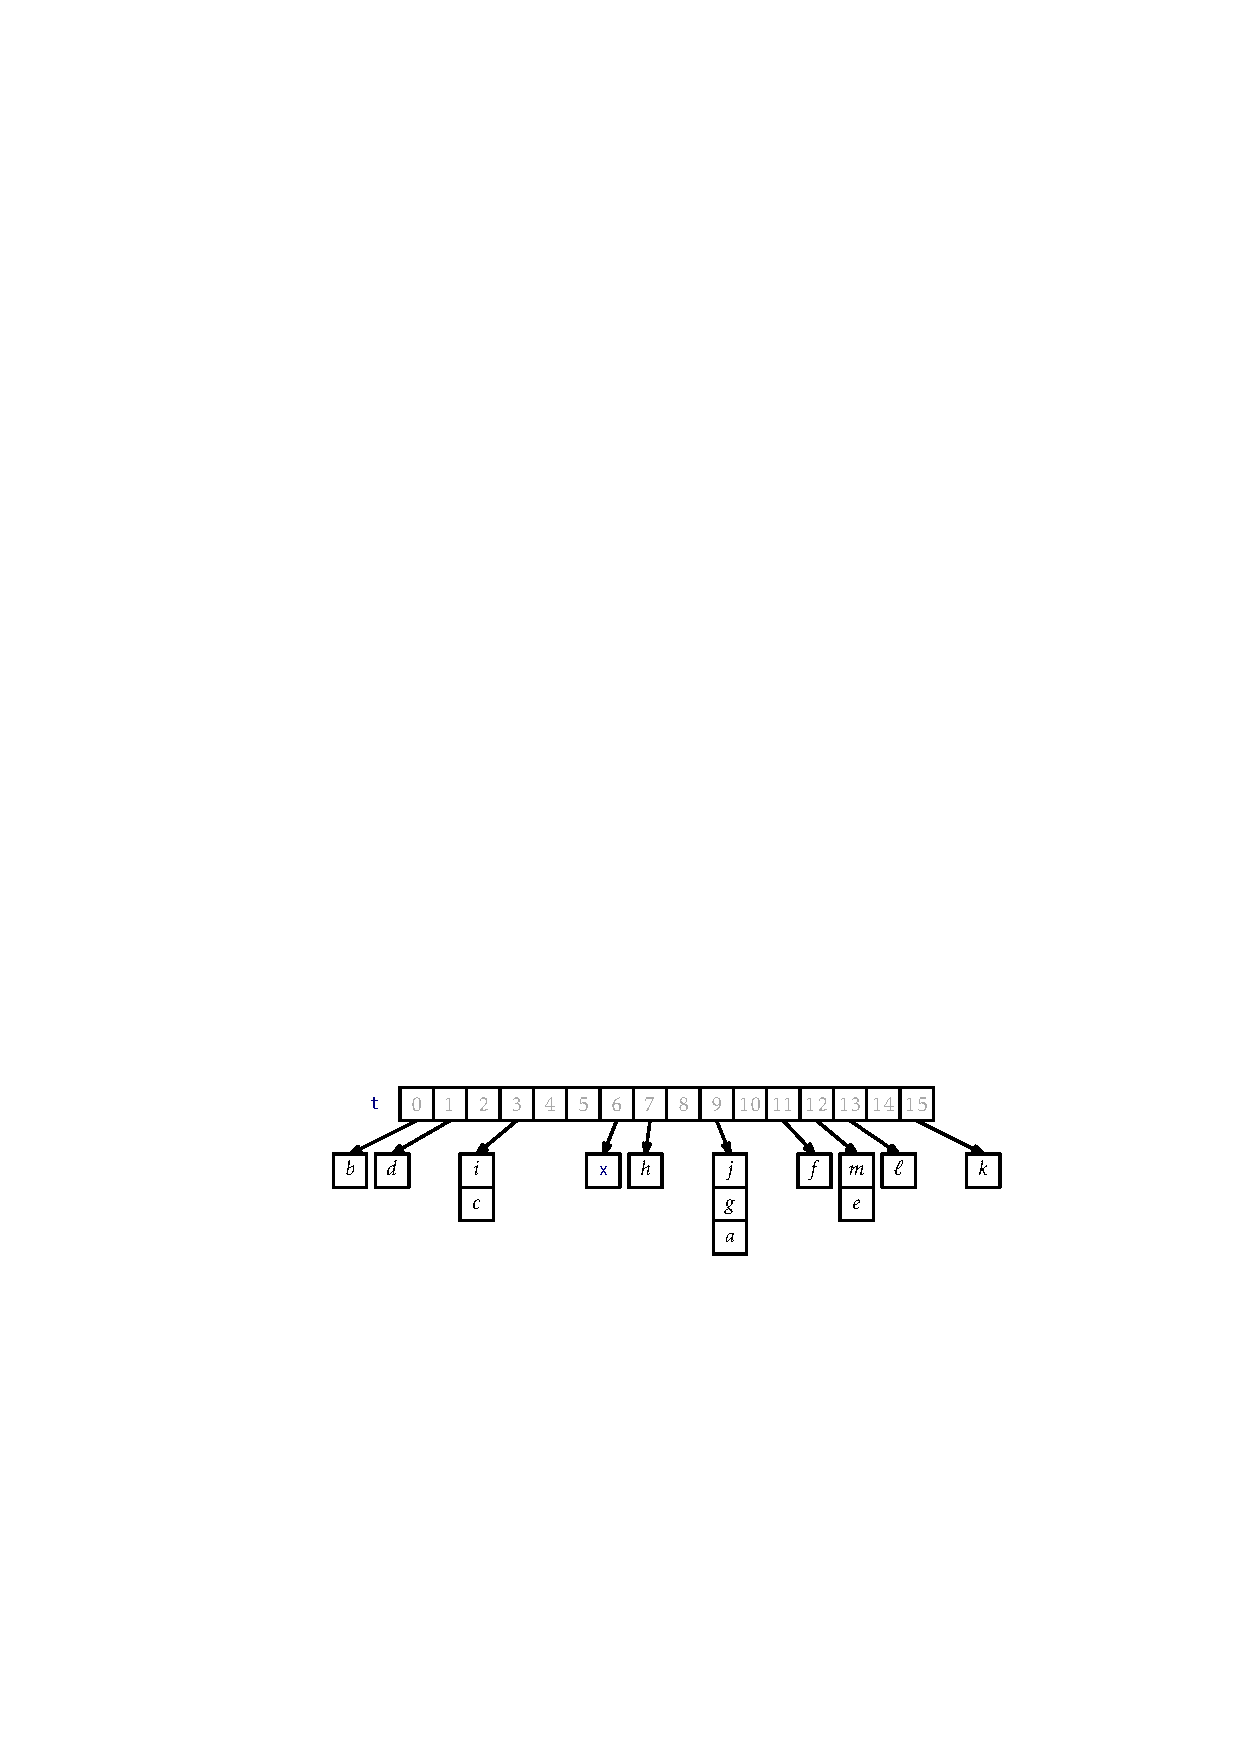
\includegraphics[width=\ScaleIfNeeded]{figs/chainedhashtable}
   \end{center}
   \caption[Uma ChainedHashTable]{Um exemplo de #ChainedHashTable# com $#n#=14$ e $#t.length#=16$. Nesse exemplo $#hash(x)#=6$}
   \figlabel{chainedhashtable}
\end{figure}
\index{hash value}%
\index{hash(x)@#hash(x)#}%
O \emph {valor hash} de um item de dados #x#, indicado por #hash(x)#, é um valor na faixa $\{0,\ldots,#t.length#-1\}$. Todos os itens com valor de hash #i# são armazenados na lista em #t[i]#. Para garantir que as listas não sejam grandes, mantemos o invariante
\[
    #n# \le #t.length#
\]
assim, a média de números armazenados na lista será 
$#n#/#t.length# \le 1$.

Para adicionar um elemento, #x#, à tabela de hash, primeiro verificamos se o comprimento de #t# precisa ser aumentado e, se assim for, crescemos #t#. Com isso resolvido, vamos decodificar #x# por meio de uma função hash para obtermos um número inteiro, #i#, no intervalo $\{0,\ldots,#t.length#-1\}$ e anexamos #x# à lista #t[i]#:
\codeimport{ods/ChainedHashTable.add(x)}
Crescer a tabela, se necessário, envolve duplicar o comprimento de #t# e reinserir todos os elementos na nova tabela. Esta estratégia é exatamente a mesma que a utilizada na implementação da #ArrayStack# e o mesmo resultado se aplica: O custo de crescimento é apenas constante quando amortizado em uma sequência de inserções (veja ~\lemref{arraystack-amortized} na página ~\pageref{lem:arraystack-amortized}).

Além de crescer, o único outro trabalho feito ao adicionar um novo valor #x# a uma #ChainedHashTable# envolve anexar #x# à lista #t[hash(x)]#. Para qualquer uma das implementações de lista descritas nos Capítulos ~\ref{chap:arrays} ou \ref{chap:linkedlists}, isso leva um tempo constante.

Para remover um elemento, #x#, da tabela hash, iteramos sobre a lista #t[hash(x)]# até encontrar #x# para, então, removê-lo:
\codeimport{ods/ChainedHashTable.remove(x)}
Isso leva $O(#n#_{#hash(x)#})$ tempo, onde $#n#_{#i#}$ indica o comprimento da lista armazenada em #t[i]#.

Procurar o elemento #x# em uma tabela de hash é semelhante. Realizamos uma pesquisa linear na lista #t[hash(x)]#:
\codeimport{ods/ChainedHashTable.find(x)}
Novamente, isso leva tempo proporcional ao comprimento da lista #t[hash(x)]#.

O desempenho de uma tabela hash depende criticamente da escolha da função hash. Uma boa função de hash irá espalhar os elementos uniformemente entre as listas #t.length#, de modo que o tamanho esperado da lista #t[hash(x)]# será $O(#n#/#t.length)# = O(1)$. Por outro lado, uma má função de hash espalhará todos os valores (incluindo #x#) para a mesma localização da tabela, caso em que o tamanho da lista #t[hash(x)]# será #n#. Na próxima seção, descrevemos uma boa função de hash.

\subsection{Hash Multiplicativo}
\seclabel{multihash}

\index{hashing!multiplicative}%
\index{multiplicative hashing}%
O hashing multiplicativo é um método eficiente de gerar valores de hash com base na aritmética modular (discutido em \secref{arrayqueue}) e na divisão de números inteiros. Ele usa o operador $\ddiv$, que calcula a parte inteira de um quociente, ao descartar o restante.
Formalmente, para qualquer número inteiro $a\ge 0$ e $b\ge 1$, $a\ddiv b = \lfloor
a/b\rfloor$.

No hash multiplicativo, usamos uma tabela hash de tamanho $2^{#d#}$ para um número inteiro #d# qualquer (chamado \emph{dimensão}). A função hash de um inteiro $#x#\in\{0,\ldots,2^{#w#}-1\}$ é
\[
    #hash(x)# = ((#z#\cdot#x#) \bmod 2^{#w#}) \ddiv 2^{#w#-#d#} \enspace .
\]
Aqui, #z# é um inteiro \emph{ímpar} escolhido aleatoriamente em
$\{1,\ldots,2^{#w#}-1\}$. Esta função de hash pode ser realizada de
forma muito eficiente observando que, por padrão, as operações em números
inteiros já são feitas em modulo $2^{#w#}$ onde $#w#$ é o número de bits
em um número inteiro. \footnote{Isso é verdadeiro para a maioria das
linguagens de programação, incluindo C, C\#, C++ e Java. Exceções
notáveis são Python e Ruby, no qual o resultado de uma operação de
números inteiros de comprimento #w#-bit fixo, é atualizado para uma representação de comprimento variável.}  (Ver
\figref{multihashing}.) Além disso, a divisão inteira por $2^{#w#-#d#}$
é equivalente a descartar os $#w#-#d#$ bits mais à direita em uma representação binária (que é implementado deslocando os bits da direita por
$#w#-#d#$ usando o operador \javaonly{#>>>#}\cpponly{#>>#}\pcodeonly{#>>#}).  \notpcode{Desta forma, o código que implementa a fórmula acima é mais simples que a própria fórmula:}
\codeimport{ods/ChainedHashTable.hash(x)}

\begin{figure}
  \begin{center}
    \resizebox{.98\textwidth}{!}{
    \setlength{\arrayrulewidth}{1pt}
    \begin{tabular}{|lr@{}r|}\hline
    $2^#w#$ (4294967296)&            #1#&#00000000000000000000000000000000# \\
    #z# (4102541685)&                   &#11110100100001111101000101110101# \\
    #x# (42) &                          &#00000000000000000000000000101010# \\
    $#z#\cdot#x#$ &             #101000#&#00011110010010000101110100110010# \\
    $(#z#\cdot#x#)\bmod 2^{#w#}$ &      &#00011110010010000101110100110010# \\
    $((#z#\cdot#x#)\bmod 2^{#w#})\ddiv 2^{#w#-#d#}$ &&
                      \multicolumn{1}{@{}l|}{#00011110#} \\\hline
    \end{tabular}}
    \setlength{\arrayrulewidth}{.4pt}
  \end{center}
  \caption{A operação de um hash multiplicativo com $#w#=32$
    e $#d#=8$.}
  \figlabel{multihashing}
\end{figure}

O lema a seguir, cuja prova é adiada até mais tarde nesta seção, mostra que o hash multiplicativo faz um bom trabalho para evitar colisões:

\begin{lem}\lemlabel{universal-hashing}
   Seja #x# e #y# dois valores em $\{0,\ldots,2^{#w#}-1\}$ com $#x#\neq #y#$. Então $\Pr\{#hash(x)#=#hash(y)#\} \le 2/2^{#d#}$.
\end{lem}

Com o \lemref{universal-hashing}, o desempenho de #remove(x)# e #find(x)# são fáceis de analisar:

\begin{lem}
  Para qualquer valor de dados #x#, o comprimento esperado da lista #t[hash(x)]# é no máximo $#n#_{#x#} + 2$, onde $#n#_{#x#}$ é o número de ocorrências de #x# na tabela hash.
\end{lem}

\begin{proof}
  Tomando $S$ pelo (multi-)conjunto de elementos armazenados na tabela hash que não são iguais a #x#. Para um elemento $#y#\in S$, define-se a variável indicadora
    \[ I_{#y#} = \left\{\begin{array}{ll}
       1 & \mbox{se $#hash(x)#=#hash(y)#$} \\
       0 & \mbox{caso contrário}
       \end{array}\right.
    \]
  E observe que, pelo \lemref{universal-hashing}, $\E[I_{#y#}] \le 2/2^{#d#}=2/#t.length#$. O comprimento esperado da lista #t[hash(x)]# é dado por:
  \begin{eqnarray*}
   \E\left[#t[hash(x)].size()#\right] &=& \E\left[#n#_{#x#} + \sum_{#y#\in S} I_{#y#}\right] \\
    &=& #n#_{#x#} + \sum_{#y#\in S} \E [I_{#y#} ] \\
    &\le& #n#_{#x#} + \sum_{#y#\in S} 2/#t.length# \\
    &\le& #n#_{#x#} + \sum_{#y#\in S} 2/#n# \\
    &\le& #n#_{#x#} + (#n#-#n#_{#x#})2/#n# \\
    &\le& #n#_{#x#} + 2 \enspace ,
  \end{eqnarray*}
  conforme exigido.
\end{proof}

Agora, queremos provar \lemref{universal-hashing}, mas primeiro precisamos de um resultado da teoria dos números. Na seguinte prova, usamos a notação $(b_r,\ldots,b_0)_2$ para denotar $\sum_{i=0}^r b_i2^i$, onde cada $b_i$ é um pouco, seja 0 ou 1. Em outras palavras, $(b_r,\ldots, b_0)_2$ é o inteiro cuja representação binária é dada por $b_r,\ldots,b_0$.
Usamos $\star$ para denotar um bit de valor desconhecido.

\begin{lem}\lemlabel{hashing-mapping}
  Seja $S$ o conjunto de inteiros ímpares em $\{1,\ldots,2^{#w#}-1\}$; Seja $q$ e $i$ dois elementos em $S$. Então há exatamente um valor $#z#\in S$, de modo que $#z#q\bmod 2^{#w#} = i$.
\end{lem}

\begin{proof}
  Uma vez que o número de escolhas para $#z#$ e $i$ é o mesmo, basta provar que existe \emph{no máximo} um valor $#z#\in S$ que satisfaça $#z#q\bmod 2^{#w#} = i$.

  Suponhamos, por uma questão de contradição, que existem dois desses valores #z# e #z'#, com $#z#>#z#'$. Então
  \[
     #z#q\bmod 2^{#w#} = #z#'q \bmod 2^{#w#} = i
  \]
  Portanto
  \[ 
     (#z#-#z#')q\bmod 2^{#w#} = 0 
  \]
  Mas isso significa que 
  \begin{equation}
    (#z#-#z#')q = k 2^{#w#} \eqlabel{factors} 
  \end{equation}
  para qualquer inteiro $k$.  Pensando em termos de números binários, temos que 
  \[
    (#z#-#z#')q = k\cdot(1,\underbrace{0,\ldots,0}_{#w#})_2 \enspace ,
  \]
  de modo que os #w# bits de fuga na representação binária de $(#z#-#z#')q$ são todos os 0's.

  Além disso, $k\neq 0$, desde $q\neq 0$ e $#z#-#z#'\neq 0$. Uma vez que $q$ é impar, não possui 0's na sua representação binária.
  \[
    q = (\star,\ldots,\star,1)_2 \enspace .
  \]
  Desde $|#z#-#z#'| < 2^{#w#}$, $#z#-#z#'$ tem menos do que # w # 0's seguidos na sua representação binária:
  \[
    #z#-#z#' = (\star,\ldots,\star,1,\underbrace{0,\ldots,0}_{<#w#})_2
      \enspace .
  \]
  Portanto, o produto $(#z#-#z#')q$ tem menos do que #w# 0's na sua representação binária:
  \[
   (#z#-#z#')q = (\star,\cdots,\star,1,\underbrace{0,\ldots,0}_{<#w#})_2 
    \enspace .
  \]
  Dessa forma, $(#z#-#z#')q$ não pode satisfazer \myeqref{factors}, produzindo uma contradição e completando a prova.
\end{proof}

A utilidade do \lemref{hashing-mapping} vem da seguinte observação: Se #z# for escolhido uniformemente aleatoriamente de $S$, então #zt# é distribuído uniformemente em $S$. Na seguinte prova, ajuda a pensar na representação binária de #z#, que consiste em $#w#-1$ bits aleatórios seguido por um 1.

\begin{proof}[Prova do \lemref{universal-hashing}]
  Primeiro, observamos que a condição $#hash(x)#=#hash(y)#$ é equivalente à declaração ``a ordem mais alta #d# bits de $#z# #x# \bmod2 ^{#w#}$ e os #d# bits de ordem superior $#z# #y#\bmod 2^{#w#}$ são os mesmos.'' Uma condição necessária dessa afirmação é que os bits #d# de ordem superior na representação binária de $#z#(#x#-#y#) \ bmod 2 ^ {# w #} $ são todos 0 ou todos 1. Isso é,
  \begin{equation}
  #z#(#x#-#y#)\bmod 2^{#w#} = 
  (\underbrace{0,\ldots,0}_{#d#},\underbrace{\star,\ldots,\star}_{#w#-#d#})_2 
  \eqlabel{all-zeros}
  \end{equation}
  quando $#zx#\bmod 2^{#w#} > #zy#\bmod 2^{#w#}$ ou
  \begin{equation}
  #z#(#x#-#y#)\bmod 2^{#w#} = 
  (\underbrace{1,\ldots,1}_{#d#},\underbrace{\star,\ldots,\star}_{#w#-#d#})_2 
  \enspace .
  \eqlabel{all-ones}
  \end{equation}
  quando $#zx#\bmod 2^{#w#} < #zy#\bmod 2^{#w#}$. Portanto, apenas temos que limitar a probabilidade de que $#z#(#x#-#y#) \bmod 2^{#w#}$ pareça \myeqref{all-zeros} ou \myeqref{all-ones}.
  
  Seja $ q $ um inteiro ímpar exclusivo tal que $(#x#-#y#)\bmod 2^{#w#}=q2^r$ para algum inteiro $r\ge 0$. Pela \lemref{hashing-mapping}, a representação binária de $#z#q\bmod 2^{#w#}$ tem $#w#-1$ bits aleatórios, seguido por um 1:
  \[
   #z#q\bmod 2^{#w#}  = (\underbrace{b_{#w#-1},\ldots,b_{1}}_{#w#-1},1)_2
  \]
  Portanto, a representação binária de $#z#(#x#-#y#)\bmod 2^{#w#}=#z#q2^r\bmod 2^{#w#}$ tem $#w#-r-1$ bits aleatórios, seguido de um 1, seguido de $r$ 0's:
  \[
  #z#(#x#-#y#)\bmod 2^{#w#}  =
  #z#q2^{r}\bmod 2^{#w#} =
      (\underbrace{b_{#w#-r-1},\ldots,b_{1}}_{#w#-r-1},1,\underbrace{0,0,\ldots,0}_{r})_2
  \]
  Agora podemos finalizar a prova: se $r > #w#-#d#$, então os #d# bits de ordem superior de $#z#(#x#-#y#)\bmod 2^{#w#}$ contêm tanto 0's quanto 1's, então a probabilidade de que $#z#(#x#-#y#)\bmod 2^{#w#}$ pareça \myeqref{all-zeros} ou \myeqref{all-ones} é 0 . Se $#r#=#w#-#d#$, então a probabilidade de se parecer com \myeqref{all-zeros} é 0, mas a probabilidade de se parecer com \myeqref{all-ones} é $1/2^{#d#-1}=2/2^{#d#}$ (uma vez que devemos ter $b_1,\ldots,b_ {d-1}=1,\ldots,1$). Se $r < #w#-#d#$, então devemos ter $b_{#w#-r-1},\ldots,b_{#w#-r-#d#}=0,\ldots,0$ ou $b_{#w#-r-1},\ldots,b_{#w#-r-#d#}=1,\ldots,1$. A probabilidade de cada um desses casos é $1/2^{#d#}$ e eles são mutuamente exclusivos, então a probabilidade de um desses casos é $2/2^{#d#}$. Isso completa a prova.
\end{proof}

\subsection{Resumo}

O seguinte teorema resume o desempenho de uma estrutura de dados #ChainedHashTable#:

\begin{thm}\thmlabel{hashtable}
  Uma #ChainedHashTable# implementa a interface #USet#. Ignorando o custo das chamadas para #grow()#, a #ChainedHashTable# suporta as operações #add(x)#, #remove(x)# e #find(x)# em $O(1)$ tempo esperado por operação.

  Além disso, começando com uma #ChainedHashTable# vazia, qualquer sequência de operações de $m$ #add(x)# e #remove(x)# resultará num total de $O(m)$ tempo gasto durante todas as chamadas para #grow()#.
\end{thm}

\section{#LinearHashTable#: Sondagem Linear}
\seclabel{linearhashtable}

\index{LinearHashTable@#LinearHashTable#}%
A estrutura de dados #ChainedHashTable# usa uma matriz de listas, onde a #i#-ésima lista armazena todos os elementos #x#, tal que $#hash(x)#=#i#$. Uma alternativa, chamada \emph{endereçamento aberto}
\index{open addressing}%
é armazenar os elementos diretamente em um array, #t#, com cada local do array em #t# armazenando no máximo um valor. Essa abordagem é tomada pela #LinearHashTable# descrita nesta seção. Em alguns lugares, esta estrutura de dados é descrita como \emph{endereçamento aberto com sondagem linear}.
\index{linear probing}%

A principal ideia por trás de uma #LinearHashTable# é que gostaríamos, de preferência, de armazenar o elemento #x# com o valor hash #i=hash(x)# na localização da tabela #t[i]#. Se não pudermos fazer isso (porque algum elemento já está armazenado), então tentamos armazená-lo na localização $#t#[(#i#+1)\bmod#t.length#]$; Se isso não for possível, tentemos $#t#[(#i#+2)\bmod#t.length#]$, e assim por diante, até encontrar um lugar para #x#.

Há três tipos de registros armazenados em #t#: 
\begin{enumerate}
  \item dados: valores reais no #USet# que estamos representando;
   \item valores #null#: em locais de matriz onde nenhum dado foi armazenado; e
   \item valores #del#: em locais de matriz onde os dados foram armazenados uma vez, mas que já foram excluídos.
\end{enumerate}
Além do contador, #n#, que acompanha o número de elementos na #LinearHashTable#, um contador, #q#, acompanha o número de elementos dos Tipos~1 e 3. Isso é, #q# é igual a #n# mais o número de #del# valores em #t#. Para que isso funcione de forma eficiente, precisamos #t# para ser consideravelmente maior do que #q#, de modo que existam muitos valores #null# em #t#. As operações na #LinearHashTable# mantêm, portanto, o invariante que $#t.length#\ge 2#q#$.

Para resumir, um #LinearHashTable# contém uma matriz, #t#, que armazena elementos de dados e números inteiros #n# e #q# que acompanham o número de elementos de dados e valores não #null# de #t#, respectivamente. Como muitas funções de hash funcionam apenas para tamanhos de tabela que são uma potência de 2, também mantemos um inteiro #d# e mantenha o invariante que $#t.length#=2^#d#$.
\codeimport{ods/LinearHashTable.t.n.q.d}

A operação #find(x)# em #LinearHashTable# é simples. Nós começamos na entrada do array #t[i]# onde $#i#=#hash(x)#$ e entradas de pesquisa #t[i]#, $#t#[(#i#+1)\bmod #t.length#]$, $#t#[(#i#+2)\bmod #t.length#]$, e assim por diante, até encontrarmos um índice #i'# tal que, também, #t[i']=x#, ou #t[i']=null#.
No primeiro caso, nós retornamos #t[i']#. No último caso, concluímos que # x # não está contido na tabela hash e retorna #null#.
\codeimport{ods/LinearHashTable.find(x)}

A operação #add(x)# também é bastante fácil de implementar. Depois de verificar que #x# ainda não está armazenado na tabela (usando #find(x)#), buscamos #t[i]#, $#t#[(#i#+1)\bmod #t.length#]$, $#t#[(#i#+2)\bmod #t.length#]$, e assim por diante, até encontrar #null# ou #del# e armazenar #x# nessa localização, incrementar #n# e #q#, se apropriado.
\codeimport{ods/LinearHashTable.add(x)}

Agora, a implementação da operação #remove (x) # deve ser óbvia.
Nós buscamos #t[i]#, $#t#[(#i#+1)\bmod #t.length#]$, $#t#[(#i#+2)\bmod #t.length#]$, e assim por diante até encontrar um índice #i'# tal que #t[i']=x# ou #t[i']=null#. No primeiro caso, definimos #t[i']=del# e retornamos #true#. No último caso, concluímos que #x# não foi armazenado na tabela (e, portanto, não pode ser excluído) e retornar #false#.
\codeimport{ods/LinearHashTable.remove(x)}

A correção dos métodos #find(x)#, #add(x)# e #remove(x)# é fácil de verificar, contudo ela se apoia no uso de valores #del#. Observe que nenhuma dessas operações nunca estabeleceu uma entrada não-#null# para #null#.
Portanto, quando alcançamos um índice #i'# tal que #t[i']=null#, esta é uma prova de que o elemento #x#, que estamos procurando, não está armazenado na tabela; #t[i']# sempre foi #null#, então não há nenhuma razão para que uma operação anterior #add(x)# tenha prosseguido além do índice #i'#.

O método #resize()# é chamado por #add(x)# quando o número de entradas não-#null# excede $#t.length#/2$ ou #remove(x)# quando o número de entradas de dados é inferior a #t.length/8#. O método #resize()# funciona como os métodos #resize()# de outras estruturas de dados baseadas em array.
Encontramos o menor inteiro não negativo #d# tal que $2^{#d#}\ge 3#n#$. Realocamos o array #t# para que ela tenha tamanho $2^{#d#}$ e, em seguida, inserimos todos os elementos da versão anterior de #t# na nova cópia redimensionada de #t#. Ao fazer isso, restabelecemos #q# igual a #n#, pois o recém-alocado #t# não contém valores #del#.
\codeimport{ods/LinearHashTable.resize()}

\subsection{Análise da Sondagem Linear}

Observe que cada operação, #add(x)#, #remove(x)# ou #find(x)#, termina assim que (ou antes que) descubra a primeira entrada #null# em #t#.
A intuição por trás da análise de sondagem linear é que, uma vez que pelo menos metade dos elementos em #t# são iguais a #null#, uma operação não demorará muito para ser concluída, pois será muito rápido encontrar uma entrada #null#. No entanto, não devemos confiar muito nessa intuição, porque isso nos levaria à conclusão (incorreta) de que o número esperado de locais em #t# examinado por uma operação é no máximo de 2.

Para o restante desta seção, assumiremos que todos os valores de hash são distribuídos de forma independente e uniforme em $\{0,\ldots,#t.length#-1\}$.
Esta não é uma suposição realista, mas permitirá que analisemos a sondagem linear. Mais tarde, nesta seção, descreveremos um método, chamado de hash de tabulação, que produz uma função de hash que é "suficientemente boa" para sondagem linear. Também assumiremos que todos os índices nas posições de #t# são tomados no módulo #t.length#, de modo que #t[i]# é realmente uma abreviatura para $#t#[#i#\bmod#t.length#]$.

\index{run}%
Dizemos que um \emph {percurso $ k $ que começa em # i #} ocorre quando todas as entradas da tabela $#t[i]#, #t[i+1]#,\ldots,#t#[#i#+k-1]$ não são #null# e $#t#[#i#-1]=#t#[#i#+k]=#null#$. O número de elementos não-#null# de #t# é exatamente #q# e o método #add (x) # garante que, em todos os momentos, $#q#\le#t.length#/2$. Existem #q# elementos $#x#_1,\ldots,#x#_{#q#}$ que foram inseridos em #t# desde a última operação #resize()#.
Por nossa suposição, cada um deles tem um valor de hash, $#hash#(#x#_j)$,
Isso é uniforme e independente do resto. Com esta configuração, podemos provar o lema principal necessário para analisar a sondagem linear.

\begin{lem}\lemlabel{linear-probing}
Corrija um valor $#i#\in\{0,\ldots,#t.length#-1\}$. Então, a probabilidade de que um período de $k$ começado em #i# seja $O(c^k)$ para alguma constante $0<c<1$.
\end{lem}

\begin{proof}
Se um período de $k$ começar em #i#, então existem exatamente $k$ elementos $#x#_j$ such that $#hash#(#x#_j)\in\{#i#,\ldots,#i#+k-1\}$.
A probabilidade de isso ocorrer é exatamente
\[
  p_k  = \binom{#q#}{k}\left(\frac{k}{#t.length#}\right)^k\left(\frac{#t.length#-k}{#t.length#}\right)^{#q#-k} \enspace ,
\]
uma vez que, para cada escolha de $k$ elementos, esses $k$ elementos devem se dispersar para um dos $k$ locais e o restante $#q#-k$ elementos devem se dispersar para os outros $#t.length#-k$ locais da tabela. \footnote{Note que $p_k$ é maior do que a probabilidade de que um percurso $k$ comece em #i#, uma vez que a definição de $p_k$ não inclui o requisito $#t#[#i#-1]=#t#[#i#+k]=#null#$.}

Na derivação a seguir, vamos trapacear um pouco e substituir $r!$ por $(r/e)^r$. A Aproximação de Stirling (\secref{factorials}) mostra que isso é apenas um fator de $O(\sqrt{r})$ da verdade. Isso é feito apenas para tornar a derivação mais simples; \excref{linear-probing} pede ao leitor para refazer o cálculo de forma mais rigorosa usando a Aproximação de Stirling na sua totalidade.

O valor de $p_k$ é máximo quando #t.length# é mínimo, e a estrutura de dados mantém a invariante de $#t.length# \ge 2#q#$, então
\begin{align*}
   p_k & \le \binom{#q#}{k}\left(\frac{k}{2#q#}\right)^k\left(\frac{2#q#-k}{2#q#}\right)^{#q#-k} \\
  & = \left(\frac{#q#!}{(#q#-k)!k!}\right)\left(\frac{k}{2#q#}\right)^k\left(\frac{2#q#-k}{2#q#}\right)^{#q#-k} \\
  & \approx \left(\frac{#q#^{#q#}}{(#q#-k)^{#q#-k}k^k}\right)\left(\frac{k}{2#q#}\right)^k\left(\frac{2#q#-k}{2#q#}\right)^{#q#-k} && \text{[Aproximação de Stirling]} \\
  & = \left(\frac{#q#^{k}#q#^{#q#-k}}{(#q#-k)^{#q#-k}k^k}\right)\left(\frac{k}{2#q#}\right)^k\left(\frac{2#q#-k}{2#q#}\right)^{#q#-k} \\
 & = \left(\frac{#q#k}{2#q#k}\right)^k
     \left(\frac{#q#(2#q#-k)}{2#q#(#q#-k)}\right)^{#q#-k} \\
 & = \left(\frac{1}{2}\right)^k
     \left(\frac{(2#q#-k)}{2(#q#-k)}\right)^{#q#-k} \\
 & = \left(\frac{1}{2}\right)^k
     \left(1+\frac{k}{2(#q#-k)}\right)^{#q#-k} \\
 & \le \left(\frac{\sqrt{e}}{2}\right)^k \enspace .
\end{align*}
(Na última etapa, usamos a desigualdade $(1+1/x)^x \le e$, que é válida para todos os $x>0$.) Como $\sqrt{e}/{2}< 0.824360636 < 1$, isso completa a prova.
\end{proof}

Usando \lemref{linear-probing} para provar limites superiores no tempo de execução esperado de #find(x)#, #add(x)# e #remove(x)# agora é bastante sucinto. Considere o caso mais simples, onde executamos #find(x)# para algum valor #x# que nunca tenha sido armazenado no #LinearHashTable#. Nesse caso, $#i#=#hash(x)#$ é um valor aleatório em $\{0,\ldots,#t.length#-1\}$ independentemente do conteúdo de #t#. Se #i# for parte de uma extensão de $k$, então o tempo necessário para executar a operação #find(x)# é no máximo $O(1+k)$. Assim, o tempo de execução esperado pode ser delimitado por
\[
  O\left(1 + \left(\frac{1}{#t.length#}\right)\sum_{i=1}^{#t.length#}\sum_{k=0}^{\infty} k\Pr\{\text{#i# é parte de uma série $k$}\}\right) \enspace .
\]
Observe que cada rodada de comprimento $k$ contribui para a soma interna $k$ vezes para uma contribuição total de $k^2$, então a soma acima pode ser reescrita como
\begin{align*}
  & { } O\left(1 + \left(\frac{1}{#t.length#}\right)\sum_{i=1}^{#t.length#}\sum_{k=0}^{\infty} k^2\Pr\{\mbox{#i# começa uma série $k$}\}\right) \\
  & \le O\left(1 + \left(\frac{1}{#t.length#}\right)\sum_{i=1}^{#t.length#}\sum_{k=0}^{\infty} k^2p_k\right) \\
  & = O\left(1 + \sum_{k=0}^{\infty} k^2p_k\right) \\
  & = O\left(1 + \sum_{k=0}^{\infty} k^2\cdot O(c^k)\right) \\
  & = O(1) \enspace .
\end{align*}
O último passo nesta derivação vem do fato de que $\sum_{k=0}^{\infty} k^2\cdot O(c^k)$ é uma série exponencialmente decrescente. \footnote{Na terminologia de muitos textos de cálculo, esta soma passa o teste de razão: existe um inteiro positivo $k_0$ tal que, para todos $k\ge k_0$, $\frac{(k+1)^2c^{k+1}}{k^2c^k} < 1$.}
Portanto, concluimos que o tempo de execução esperado da operação #find(x)# para um valor #x# que não está contido em #LinearHashTable# é $O(1)$.

Se ignorarmos o custo da operação #resize()#, a análise acima nos dá tudo o que precisamos para analisar o custo das operações em um #LinearHashTable#.

Em primeiro lugar, a análise de #find(x)# fornecida acima aplica-se à operação #add(x)# quando #x# não está contido na tabela. Para analisar a operação #find(x)# quando #x# estiver contida na tabela, precisamos apenas observar que isso é o mesmo que o custo da operação #add(x)# que adicionou #x# na tabela anterior. Finalmente, o custo de uma operação #remove(x)# é igual ao custo de uma operação #find(x)#.

Em resumo, se ignorarmos o custo das chamadas para #resize()#, todas as operações em #LinearHashTable# são executadas em $O(1)$ tempo esperado. A contabilização do custo do redimensionamento pode ser feita usando o mesmo tipo de análise amortizada realizada para a estrutura de dados #ArrayStack# em \secref{arraystack}.

\subsection{Resumo}

O seguinte teorema resume o desempenho da estrutura de dados #LinearHashTable#:

\begin{thm}\thmlabel{linear-probing}
  A #LinearHashTable# implementa a interface #USet#. Ignorando o custo das chamadas para #resize()#, #LinearHashTable# suporta as operações #add(x)#, #remove(x)# e #find(x)# em $O(1)$ tempo esperado por operação.

  Além disso, começando uma #LinearHashTable# vazia, qualquer sequência de $m$ #add(x)# e #remove(x)# operações resulta em um total de $O(m)$ tempo gasto durante todas as chamadas para #resize()#.
\end{thm}

\subsection{Hashing por Tabulação}%Não sei se Tabulação por Dispersão seria melhor
\seclabel{tabulation}

\index{tabulation hashing}%
Ao analisar a estrutura # LinearHashTable #, fizemos uma suposição muito forte: que para qualquer conjunto de elementos, $\{#x#_1,\ldots,#x#_#n#\}$, os valores de hash $#hash#($x$_1),\ldots,#hash#(#x#_#n#)$ são distribuídos de forma independente e uniforme sobre o conjunto $\{0,\ldots,#t.length#-1\}$. Uma maneira de conseguir isso é armazenar em um array gigante, #tab#, de comprimento $2^{#w#}$, onde cada entrada é um inteiro de #w#-bit aleatório, independente de todas as outras entradas. Desta forma, podemos implementar #hash(x)# extraindo um inteiro de #d#-bit de #tab[x.hashCode()]#:
\codeimport{ods/LinearHashTable.idealHash(x)}
\pcodeonly{Aqui, #>>#, é o operador \emph{deslocamento de bits para a direita}, então
	 \begin{center}
	 	#x.hashCode() >> w-d# 
	 \end{center}
extrai os #d# bits mais significativos de #x#'s de #w#-bit códigos hash.}

Infelizmente, armazenar uma matriz de tamanho $2^{#w#}$ é proibitivo em termos de uso de memória. A abordagem usada por \emph {tabulação hashing} é, em vez disso, tratar números # w #-bit como sendo compostos de $#w#/#r#$ inteiros, cada um com apenas $#r#$ bits. Desta forma, o hashing de tabulação só precisa de $#w#/#r#$ arrays cada um do comprimento $2^{#r#}$. Todas as entradas nesses arrays são #w#-bit inteiros aleatoriamente independentes. Para obter o valor de #hash(x)#, divide-se os números inteiros #x.hashCode()# em $#w#/#r#$ #r#-bit e usamos estes como índices nesses arrays. Em seguida, combinamos todos esses valores com o operador exclusivo de bit a bit para obter #hash(x)#.
O código a seguir mostra como isso funciona quando $#w#=32$ e $#r#=4$:
\codeimport{ods/LinearHashTable.hash(x)}
Nesse caso, # tab # é um array bidimensional com quatro colunas e $2^{32/4}=256$ linhas.
\pcodeonly{
Quantidades como #0xff#, usadas acima, são \emph{números hexadecimais}
\index{hexadecimal numbers}%
cujos dígitos têm 16 valores possíveis 0--9, que têm seu significado usual e a-f, que denotam 10--15. O número $#0xff#=15\cdot 16 + 15 = 255$. O símbolo #&# é o operador \emph{bitwise AND}, então codifique como #h >> 8 & 0xff# extrai bits com índice 8 a 15 de #h#.}

Pode-se verificar facilmente que, para qualquer #x#, #hash(x)# é uniformemente distribuído em $\{0,\ldots,2^{#d#}-1\}$. Com um pouco de trabalho, pode-se verificar se qualquer par de valores possui valores de hash independentes. Isso implica que o hash de tabulação poderia ser usado em lugar de hashing multiplicativo para a implementação #ChainedHashTable#.

No entanto, não é verdade que qualquer conjunto de #n# valores distintos forneça um conjunto de valores de hash independentes #n#. Contudo, quando o hashing de tabulação é usado, o limite de \thmref{linear-probing} ainda é válido. Referências para isso são fornecidas no final deste capítulo.

\section{Hash Codes}

\index{hash code}%
As tabelas de hash discutidas na seção anterior são usadas para associar dados com chaves inteiras consistindo de #w# bits. Em muitos casos, temos chaves que não são inteiros. Podem ser cordas, objetos, arrays ou outras estruturas compostas. Para usar tabelas de hash para esses tipos de dados, devemos mapear esses tipos de dados para os códigos de hash #w#-bit. Os mapeamentos de código Hash devem ter as seguintes propriedades:

\begin{enumerate}
  \item Se #x# e #y# forem iguais, então #x.hashCode()# e #y.hashCode()# são iguais.

  \item Se #x# e #y# não forem iguais, então a probabilidade de que $#x.hashCode()#=#y.hashCode()#$ sejam iguais deve ser pequena (perto de $1/2^{#w#}$).
\end{enumerate}

A primeira propriedade garante que, se armazenarmos #x# em uma tabela hash e, mais tarde, procuremos um valor #y# igual a #x#, então encontraremos #x# --- como deveríamos.
A segunda propriedade minimiza a perda de converter nossos objetos em números inteiros. Ele garante que os objetos desiguais geralmente tenham códigos de hash diferentes e, portanto, provavelmente serão armazenados em locais diferentes em nossa tabela de hash.

\subsection{Códigos Hash para Tipos Primitivos de Dados}

\index{hash code!for primitive data}%
Pequenos tipos de dados primitivos, como #char#, #byte#, #int# e #float# ,geralmente, são fáceis de encontrar códigos de hash. Esses tipos de dados sempre têm uma representação binária e essa representação binária geralmente consiste em #w# ou menos bits. \javaonly{(Por exemplo, em Java, #byte# é um tipo de 8 bits e #float# é um tipo de 32 bits.)}\cpponly{(Por exemplo, em C ++ #char# geralmente é um tipo de 8 bits e #float# é um tipo de 32 bits).} Nesses casos, tratamos esses bits como a representação de um número inteiro na faixa $\{0,\ldots,2^#w#-1\}$ . Se dois valores são diferentes, eles obtêm códigos hash diferentes. Se eles são o mesmo, eles obtêm o mesmo código hash.

Alguns tipos de dados primitivos são compostos por mais de #w# bits, geralmente $c#w#$ bits para algum inteiro constante $c$. (Os tipos #long# e #double# do Java são exemplos disso com $c=2$.) Esses tipos de dados podem ser tratados como objetos compostos feitos de $c$ partes, conforme descrito na próxima seção.

\subsection{Códigos Hash para Objetos Compostos}
\seclabel{stringhash}

\index{hash code!for compound objects}%
Para um objeto composto, queremos criar um código hash combinando os códigos hash individuais das partes constituintes do objeto. Isso não é tão fácil quanto parece. Embora se possa encontrar muitos hacks para isso (por exemplo, combinando os códigos de hash com operações bitwise ou-exclusivo), muitos desses hacks acabam por ser fáceis de imprimir (ver exercícios ~\ref{exc:hash-hack-first}--\ref{exc:hash-hack-last}).No entanto, se alguém estiver disposto a fazer aritmética com $2# w#$ bits de precisão, existem métodos simples e robustos disponíveis. Suponha que possamos ter um objeto composto por várias partes $P_0,\ldots,P_{r-1}$ cujos códigos hash são $#x#_0,\ldots,#x#_{r-1}$. Então, podemos escolher #w#-bits inteiros aleatórios e mutuamente independentes $#z#_0,\ldots,#z#_{r-1}$ e um $2#w#$-bit inteiro impar #z# e, então, calcular um código hash para nosso objeto com
\[
   h(#x#_0,\ldots,#x#_{r-1}) =  
   \left(\left(#z#\sum_{i=0}^{r-1} #z#_i #x#_i\right)\bmod 2^{2#w#}\right)
   \ddiv 2^{#w#} \enspace .
\]
Observe que este código hash tem um passo final (multiplicando por #z# e dividindo por $2^{#w#}$) que usa a função de hash multiplicativa de \secref{multihash} para tirar o $2#w#$-bit resultado intermediário e reduzi-lo para um resultado final de #w#-bit. Aqui está um exemplo desse método aplicado a um objeto composto simples com três partes #x0#, #x1#, and #x2#:
\javaimport{junk/Point3D.x0.hashCode()}
\cppimport{ods/Point3D.hashCode()}
\pcodeimport{ods/Point3d.hashCode()}
O seguinte teorema mostra que, além de ser direto para implementar, esse método provavelmente é bom:

\begin{thm}\thmlabel{multihash}
Sejam $#x#_0,\ldots,#x#_{r-1}$ e $#y#_0,\ldots,#y#_{r-1}$ sequencias de #w# bit inteiros em $\{0,\ldots,2^{#w#}-1\}$ e assumindo $#x#_i \neq #y#_i$ para pelo menos um índice $i\in\{0,\ldots,r-1\}$. Então 
\[
   \Pr\{ h(#x#_0,\ldots,#x#_{r-1}) =  h(#y#_0,\ldots,#y#_{r-1}) \} 
        \le 3/2^{#w#} \enspace .  
\] 
\end{thm}

\begin{proof}
  Primeiro, ignoraremos o passo de hashing multiplicativo final e veremos como essa etapa contribui mais tarde. Definir:
  \[
    h'(#x#_0,\ldots,#x#_{r-1}) =  
       \left(\sum_{j=0}^{r-1} #z#_j #x#_j\right)\bmod 2^{2#w#} \enspace .
  \]
  Suponhamos que $h'(#x#_0,\ldots,#x#_{r-1}) =  h'(#y#_0,\ldots,#y#_{r-1})$.
  Podemos reescrever isso como:
  \begin{equation}  \eqlabel{bighash-x}
      #z#_i(#x#_i-#y#_i) \bmod 2^{2#w#} = t
  \end{equation}
  onde 
  \[
     t = \left(\sum_{j=0}^{i-1} #z#_j(#y#_j-#x#_j) + \sum_{j=i+1}^{r-1} #z#_j(#y#_j-#x#_j)\right) \bmod 2^{2#w#}
  \]
  Se assumirmos, sem perda de generalidade, que $#x#_i> #y#_i$, então
  \myeqref{bighash-x} se torna
  \begin{equation}
      #z#_i(#x#_i-#y#_i) = t \eqlabel{bighash-xx} \enspace ,
  \end{equation}
  já que cada $#z#_i$ e $(#x#_i-#y#_i)$ é ao menos $2^{#w#}-1$, então o produto deles é ao menos $2^{2#w#}-2^{#w#+1}+1 < 2^{2#w#}-1$.
  Pressuposto, $#x#_i-#y#_i\neq 0$, então \myeqref{bighash-xx} tem ao menos uma solução em $#z#_i$.  Portanto, uma vez que $#z#_i$ e $t$ são independentes $#z#_0,\ldots,#z#_{r-1}$ são mutuamente independentes), a probabilidade de selecionar $h'(#x#_0,\ldots,#x#_{r-1})=h'(#y#_0,\ldots,#y#_{r-1})$ seja no máximo $1/2^{#w#}$.

  O passo final da função hash é aplicar o hashing multiplicativo para reduzir o resultado  intermediário $h'(#x#_0,\ldots,#x#_{r-1})$ de $2#w#$-bit para resultado final $h(#x#_0,\ldots,#x#_{r-1})$ de #w#-bit. Pelo \thmref{multihash},
  se $h'(#x#_0,\ldots,#x#_{r-1})\neq h'(#y#_0,\ldots,#y#_{r-1})$, então
  $\Pr\{h(#x#_0,\ldots,#x#_{r-1}) = h(#y#_0,\ldots,#y#_{r-1})\} \le 2/2^{#w#}$.

  Resumindo, 
  \begin{align*}
    & \Pr\left\{\begin{array}{l}
          h(#x#_0,\ldots,#x#_{r-1}) \\
          \quad = h(#y#_0,\ldots,#y#_{r-1})\end{array}\right\} \\
      &= \Pr\left\{\begin{array}{ll}
            \mbox{$h'(#x#_0,\ldots,#x#_{r-1}) = h'(#y#_0,\ldots,#y#_{r-1})$ or} \\
            \mbox{$h'(#x#_0,\ldots,#x#_{r-1}) \neq h'(#y#_0,\ldots,#y#_{r-1})$} \\
                 \quad  \mbox{and
$#z#h'(#x#_0,\ldots,#x#_{r-1})\ddiv2^{#w#} = #z# h'(#y#_0,\ldots,#y#_{r-1})\ddiv 2^{#w#}$}
          \end{array}\right\} \\
      &\le 1/2^{#w#} + 2/2^{#w#} = 3/2^{#w#} \enspace . \qedhere
  \end{align*}
\end{proof}


\index{hash code!for strings}%
\index{hash code!for arrays}%
\subsection{Códigos Hash para Arrays e Strings}
\seclabel{polyhash}

O método da seção anterior funciona bem para objetos que possuem um número fixo, constante, de componentes. No entanto, ele se destrói quando queremos usá-lo com objetos que possuem uma quantidade variável de componentes, uma vez que requer um número aleatório $#z#_i$ de #w#-bit para cada componente. Poderíamos usar uma sequência pseudo-randômica para gerar tantos $#z#_i$'s quanto precisássemos, mas então os $#z#_i$ não seriam mutuamente independentes e, assim, torna-se-ia difícil provar que os números de pseudo-randômicos não interagem bem com a função hash que estamos usando. Em particular, os valores de $t$ e $#z#_i$ na prova de \thmref{multihash} não são mais independentes.

\index{prime field}%
Uma abordagem mais rigorosa é basear nossos códigos de hash em polinômios sobre os campos principais; Estes são apenas polinômios regulares que são avaliados em um número primo, #p#. Este método baseia-se no seguinte teorema, que diz que os polinômios sobre os campos principais se comportam quase como os polinômios usuais:

\begin{thm}\thmlabel{prime-polynomial}
 Seja $#p#$ um número primo, e seja $f(#z#) = #x#_0#z#^0 + #x#_1#z#^1 +
 \cdots + #x#_{r-1}#z#^{r-1}$ uma expressão polinomial, não trivial, com coeficientes $#x#_i\in\{0,\ldots,#p#-1\}$. Então a equação $f(#z#)\bmod #p# = 0$
 tem no mínimo $r-1$ soluções para $#z#\in\{0,\ldots,p-1\}$.
\end{thm}

Para usar o \thmref{prime-polynomial}, nós "hasheamos" uma sequência de inteiros
$#x#_0,\ldots,#x#_{r-1}$ com cada $#x#_i\in \{0,\ldots,#p#-2\}$ usando um inteiro aleatório $#z#\in\{0,\ldots,#p#-1\}$ via fórmula
\[
   h(#x#_0,\ldots,#x#_{r-1}) 
    = \left(#x#_0#z#^0+\cdots+#x#_{r-1}#z#^{r-1}+(#p#-1)#z#^r \right)\bmod #p# \enspace .
\]

Observe o termo extra $(#p#-1)#z#^r$ no final da fórmula. Isso ajuda a pensar em $(#p#-1)$ como o último elemento, $#x#_r$, na sequência $#x#_r$. Observe, também, que este elemento difere de qualquer outro elemento na sequência (cada um dos quais está no conjunto $\{0,\ldots,#p#-2\}$). Podemos pensar em $#p#-1$ como um marcador de fim de sequência.

O seguinte teorema, que considera o caso de duas sequências do mesmo comprimento, mostra que esta função hash dá um bom retorno para a pequena quantidade de aleatorização necessária para escolher #z#:

\begin{thm}\thmlabel{stringhash-eqlen}
  Seja $#p#>2^{#w#}+1$ um primo, seja $#x#_0,\ldots,#x#_{r-1}$ e
  $#y#_0,\ldots,#y#_{r-1}$ sequências de inteiros de #w#-bit em
  $\{0,\ldots,2^{#w#}-1\}$, e assumindo-se $#x#_i \neq #y#_i$ para pelo menos um índice $i\in\{0,\ldots,r-1\}$. Então
  \[
     \Pr\{ h(#x#_0,\ldots,#x#_{r-1}) =  h(#y#_0,\ldots,#y#_{r-1}) \} 
          \le (r-1)/#p# \enspace .  
  \] 
\end{thm}

\begin{proof}
  A equação $h(#x#_0,\ldots,#x#_{r-1}) =  h(#y#_0,\ldots,#y#_{r-1})$ pode ser reescrita como
  \begin{equation}  \eqlabel{strhash-eqlen}
    \left(
       (#x#_0-#y#_0)#z#^0+\cdots+(#x#_{r-1}-#y#_{r-1})#z#^{r-1} 
    \right)\bmod #p# = 0.
  \end{equation}
  Sendo $#x#_#i#\neq #y#_#i#$, um polinômio não trivial.  Portanto, pelo \thmref{prime-polynomial}, tem no máximo $r-1$ soluções em #z#. A probabilidade de escolher #z# para ser uma dessas soluções é, portanto, no máximo $(r-1)/#p#$.
\end{proof}

Note-se que esta função de hash também trata do caso em que duas sequências têm comprimentos diferentes, mesmo quando uma das sequências é um prefixo do outro. Isso ocorre porque esta função efetivamente colmeia a sequência infinita
\[
  #x#_0,\ldots,#x#_{r-1}, #p#-1,0,0,\ldots \enspace .
\]
Isso garante que, se tivermos duas sequências de comprimento $r$ e $r'$ com $r>r'$, essas duas sequências diferem no índice $i=r$. Nesse caso, \myeqref{strhash-eqlen} se torna
\[
  \left(
     \sum_{i=0}^{i=r'-1}(#x#_i-#y#_i)#z#^i + (#x#_{r'} - #p# + 1)#z#^{r'}
     +\sum_{i=r'+1}^{i=r-1}#x#_i#z#^i + (#p#-1)#z#^{r}
  \right)\bmod #p# = 0 \enspace ,
\]
que, pelo \thmref{prime-polynomial}, tem no máximo $r$ soluções em $#z#$. Isto combinado com \thmref{stringhash-eqlen} é suficiente para comprovar o seguinte teorema mais geral:

\begin{thm}\thmlabel{stringhash}
  Seja $#p#>2^{#w#}+1$ um primo, seja $#x#_0,\ldots,#x#_{r-1}$ e
  $#y#_0,\ldots,#y#_{r'-1}$ sequências distintas de inteiros de #w#-bit em
  $\{0,\ldots,2^{#w#}-1\}$. Então
  \[
     \Pr\{ h(#x#_0,\ldots,#x#_{r-1}) =  h(#y#_0,\ldots,#y#_{r-1}) \} 
          \le \max\{r,r'\}/#p#  \enspace .  
  \] 
\end{thm}

O código de exemplo a seguir mostra como esta função hash é aplicada a um objeto que contém um array, # x #, de valores:
\javaimport{junk/GeomVector.hashCode()}
\cppimport{ods/GeomVector.hashCode()}
\pcodeimport{ods/GeomVector.hashCode()}

O código anterior sacrifica alguma probabilidade de colisão para conveniência de implementação. Em particular, aplica a função hash multiplicativa de \secref{multihash}, com $#d#=31$ para reduzir #x[i].hashCode()# para um valor de 31 bits. Isto é para que as adições e multiplicações que são feitas modulo o principal $#p#=2^{32}-5$ podem ser realizadas usando aritmética não assinada de 63 bits. Assim, a probabilidade de duas sequências diferentes, cujo maior comprimento é $r$, tendo o mesmo código de hash no máximo
\[
    2/2^{31} + r/(2^{32}-5)
\]
em vez de $r/(2^{32}-5)$ especificado em \thmref{stringhash}.

\section{Discussões e Exercícios}

As tabelas Hash e os códigos hash representam um campo de pesquisa enorme e ativo que é apenas abordado neste capítulo. A Bibliografia on-line sobre Hashing \ cite {hash}
\index{Bibliografia sobre Hashing}%
contém cerca de 2000 entradas.

Existe uma variedade de implementações de tabela hash diferentes. O descrito em \secref{hashtable} é conhecido como \emph{hashing com encadeamento}
\index{hashing with chaining}%
(cada entrada do array contém uma cadeia (#List#) de elementos). Hashing com encadeamento remonta a um memorando interno da IBM criado por H. P. Luhn e datado de janeiro de 1953. Este memorando também parece ser uma das primeiras referências às linked lists.

\index{open addressing}%
Uma alternativa ao hashing com encadeamento é a usada pelos esquemas \emph{open address}, onde todos os dados são armazenados diretamente em um array. Esses esquemas incluem a estrutura # LinearHashTable # de \secref{linearhashtable}. Essa idéia também foi proposta, independentemente, por um grupo da IBM na década de 1950. Os esquemas de endereçamento aberto devem lidar com o problema de \emph{resolução de colisão}:
\ index {collision resolution}%
o caso em que dois valores hash para o mesmo local da matriz. Existem estratégias diferentes para resolução de colisão; Estes fornecem garantias de desempenho diferentes e muitas vezes exigem funções de hash mais sofisticadas do que as descritas aqui.

Outra categoria de implementações de tabela de hash são os chamados métodos de
\emph{hashing perfeito}.
\index{perfect hashing}%
Estes são métodos em que as operações #find(x)# levam $O(1)$ tempo no pior caso. Para conjuntos de dados estáticos, isso pode ser conseguido encontrando \emph {funções de hash perfeitas}
\index{perfect hash function}%
\index{hash function!perfect}%
para os dados; Essas são funções que mapeiam cada peça de dados para um local de matriz exclusivo. Para os dados que mudam ao longo do tempo, os métodos de hash perfeitos incluem \emph{tabelas de hash de dois níveis FKS}
\index{two-level hash table}%
\index{hash table!two-level}%
\cite{fks84,dkkmrt94}
e \emph{cuckoo hashing} \cite{pr04}.
\index{cuckoo hashing}%
\index{hash table!cuckoo}%

As funções de hash apresentadas neste capítulo estão provavelmente entre os métodos mais práticos atualmente conhecidos que podem comprovadamente funcionar bem para qualquer conjunto de dados. Outros métodos provavelmente bons datam do trabalho pioneiro de Carter e Wegman, que introduziram a noção de \emph{hash universal}
\index{hash universal}%
\index{hashing!universal}%
e descreveram várias funções de hash para diferentes cenários \cite{cw79}.
Hashing por tabulação, descrito em \secref{tabulation}, é graças a Carter e Wegman \cite{cw79}, mas sua análise, quando aplicada a sondagem linear (e vários outros esquemas de tabela de hash), é graças a P\v{a}tra\c{s}cu e
Thorup \cite{pt12}.

A ideia do \emph{hash multiplicativo}
\index{hash multiplicativo}%
\index{hashing!multiplicativo}%
é muito antiga e parece ser parte do folclore hashing \cite[Section~6.4]{k97v3}. No entanto, a idéia de escolher o multiplicador #z# para ser um número aleatório \emph{impar} e a análise em \secref{multihash} é devida a Dietzfelbinger \etal\
\cite{dhkp97}.  Esta versão do hashing multiplicativo é uma das mais simples, mas a probabilidade de colisão de $2/2^{#d#}$ é um fator de dois maiores do que o que se poderia esperar com uma função aleatória de $2^{#w#}\to
2^{#d#}$.  O método \emph{multiply-add hashing}
\index{hashing!multiply-add}%
\index{multiply-add hashing}%
 usa a função
\[
   h(#x#) = ((#z##x# + b) \bmod 2^{#2w#}) \ddiv 2^{#2w#-#d#}
\]
onde #z# e #b# são escolhidos aleatoriamente de $\{0,\ldots,2^{#2w#}-1\}$. O hashing Multiply-add tem uma probabilidade de colisão de apenas $1/2^{#d#}$\cite{d96}, mas requer aritmética de precisão $2#w#$-bit.

Há uma série de métodos para obter códigos hash de sequências de comprimento fixo de #w#-bit inteiros. Um método particularmente rápido
\cite{bhkkr99} é a função
\[\begin{array}{l}
  h(#x#_0,\ldots,#x#_{r-1}) \\
   \quad = \left(\sum_{i=0}^{r/2-1} ((#x#_{2i}+#a#_{2i})\bmod 2^{#w#})((#x#_{2i+1}+#a#_{2i+1})\bmod 2^{#w#})\right) \bmod 2^{2#w#}
\end{array}
\]
onde $r$ é igual e $#a#_0,\ldots,#a#_{r-1}$ são escolhidos aleatoriamente de $\{0,\ldots,2^{#w#}\}$. Isso produz um código hash de $2#w#$-bit com probabilidade de colisão $1/2^{#w#}$. Isso pode ser reduzido para um código hash de #w#-bit usando o hashing multiplicativo (ou multiplicativo). Esse método é rápido porque requer apenas $r/2$ $2#w#$-bit multiplicações , enquanto o método descrito em \secref{stringhash} requer $r$ multiplicações. (As operações $\bmod$ ocorrem implicitamente usando a aritmética #w# e $2#w#$-bit para as adições e multiplicações, respectivamente.)

O método de \secref{polyhash} de usar polinômios sobre campos primos para matrizes de comprimento variável de hash e strings é devido a Dietzfelbinger \etal\
\cite{dgmp92}. Devido ao uso do operador $\bmod$ que depende de uma instrução de máquina dispendiosa, infelizmente não é muito rápido. Algumas variantes deste método escolhem o primo #p # para ser um da forma $2^{#w#}-1$, caso em que o operador $\bmod$ pode ser substituído por adição (#+#) e operações bitwise-E (#&#) \cite[Seção~3.6]{k97v2}.
Outra opção é aplicar um dos métodos rápidos para sequências de caracteres de comprimento fixo para blocos de comprimento $c$ para alguma constante $c>1$ e, em seguida, aplicar o método de campo primário à sequência resultante de $\lceil r/c\rceil$ códigos hash.


\begin{exc}
  Uma determinada universidade atribui cada um dos números de seus alunos a primeira vez que se inscreveram para qualquer curso. Esses números são números inteiros sequenciais que começaram em 0 há muitos anos e agora estão em milhões. Suponhamos que tenhamos uma classe de alunos do primeiro ano e queremos atribuir-lhes códigos hash com base nos números de seus alunos. Faz mais sentido usar os dois primeiros dígitos ou os dois últimos dígitos do número do estudante? Justifique sua resposta.
\end{exc}

\begin{exc}
	Considere o esquema de hashing na \secref{multihash}, e suponha
	$#n#=2^{#d#}$ e $#d#\le #w#/2$.
  \begin{enumerate}
  	\item Mostre que, para qualquer escolha do multiplicador, #z#, existe #n# valores que possuem o mesmo código de hash. (Sugestão: isso é fácil e não exige nenhuma teoria de números).
     \item Dado o multiplicador, #z#, descreva #n# valores de modo que todos tenham o mesmo código de hash. (Sugestão: isto é mais difícil e requer uma teoria básica de números).
   \end{enumerate}
\end{exc}

\begin{exc}
  Prove que o limite $2/2^{#d#}$ no \lemref {universal-hashing} seja o melhor limite possível mostrando que, se $x=2^{#w#-#d#-2}$ e $#y#=3#x#$, então$\Pr\{#hash(x)#=#hash(y)#\}=2/2^{#d#}$. (Observe as representações binárias de $#zx#$ e $#z#3#x#$, e use o fato de que $#z#3#x# = #z#x#+2#z#x#$.)
\end{exc}

\begin{exc}\exclabel{linear-probing}
  Prove novamente o \lemref{linear-probing} usando a versão completa da Aproximação de Stirling dada em \secref{factorials}.
\end{exc}

\begin{exc}
  Considere a seguinte versão simplificada do código para adicionar um elemento #x# a um #LinearHashTable#, que simplesmente armazena #x# na primeira entrada #null# do array encontrada. Explique por que isso pode ser muito lento, dando um exemplo de uma sequência de $O(#n#)$ #add(x)#, #remove(x)# e #find(x)# operações que levariam na ordem de $#n#^2$ tempo de executar.
\codeimport{ods/LinearHashTable.addSlow(x)}
\end{exc}

\begin{exc}
  Versões iniciais do método Java #hashCode()# para a classe #String# trabalhada ao não usar todos os caracteres encontrados em strings longos. Por exemplo, para uma sequência de dezesseis caracteres, o código hash foi computado usando apenas os oito caracteres de índices pares. Explique por que esta foi uma idéia muito ruim dando um exemplo de grande conjunto de strings que todos têm o mesmo código hash.
\end{exc}

\begin{exc}\exclabel{hash-hack-first}
  Suponha que você tenha um objeto composto por dois números #w#-bit, #x# e #y#. Mostre porque $#x#\oplus#y#$ não faz um bom código hash para o seu objeto.
   Dê um exemplo de um grande conjunto de objetos que todos teriam código hash 0.
\end{exc}

\begin{exc}
  Suponha que você tenha um objeto composto por dois números #w#-bit, #x# e #y#. Mostre porque $#x#+#y#$ não faz um bom código hash para o seu objeto. Dê um exemplo de um grande conjunto de objetos que todos teriam o mesmo código hash.
\end{exc}

\begin{exc}\exclabel{hash-hack-last}
  Suponha que você tenha um objeto composto por dois números #w#-bit, #x# e #y#. Suponha que o código hash para seu objeto seja definido por alguma função determinística $h(#x#,#y#)$ que produz um inteiro #w#-bit inteiro. Prove que exista um grande conjunto de objetos que tenham o mesmo código hash.
\end{exc}

\begin{exc}
  Seja $p=2^{#w#}-1$ para algum inteiro positivo #w#.  Explique porque, para um inteiro positivo $x$
  \[
      (x\bmod 2^{#w#}) + (x\ddiv 2^{#w#}) \equiv x \bmod (2^{#w#}-1) \enspace .
  \]
  (Isso nos dá um algoritmo $x \bmod (2^{#w#}-1)$ para repetidamente "settar"
  \javaonly{\[
    #x = x&((1<<w)-1) + x>>>w#
  \]}
  \cpponly{\[
    #x = x&((1<<w)-1) + x>>w#
  \]}
  até $#x# \le 2^{#w#}-1$.)
\end{exc}

\begin{exc}
  Encontre algumas implementações de tabelas hash comumente usadas, tais como as implementações \javaonly{Java
  Collection Framework #HashMap#}\cpponly{The C++ STL #unordered\_map#} ou #HashTable# ou #LinearHashTable# neste livro e crie uma programa que armazena inteiros nesta estrutura de dados de modo que haja números inteiros, #x#, de modo que #find(x)# demore tempo linear. Ou seja, encontre um conjunto de #n# inteiros para os quais existem $c#n#$ elementos que dispersem para o mesmo local da tabela.

  Dependendo de quão boa seja a implementação, você poderá fazer isso apenas inspecionando o código para a implementação, ou talvez seja necessário que escreva algum código que faça inserções e pesquisas de teste, medindo quanto tempo demora para adicionar e encontrar valores específicos . (Isso pode ser, e tem sido usado, para lançar ataques de negação de serviço em servidores web \cite{cw03}.)
  \index{algorithmic complexity attack}%
\end{exc}
